\documentclass{article}


% if you need to pass options to natbib, use, e.g.:
% \PassOptionsToPackage{numbers, compress}{natbib}
% before loading nips_2016
%
% to avoid loading the natbib package, add option nonatbib:
% \usepackage[nonatbib]{nips_2016}

%\usepackage{nips_2016}

% to compile a camera-ready version, add the [final] option, e.g.:
\usepackage[final]{nips_2016}

\usepackage[utf8]{inputenc} % allow utf-8 input
\usepackage[T1]{fontenc}    % use 8-bit T1 fonts
\usepackage{hyperref}       % hyperlinks
\usepackage{url}            % simple URL typesetting
\usepackage{booktabs}       % professional-quality tables
\usepackage{amsfonts}       % blackboard math symbols
\usepackage{nicefrac}       % compact symbols for 1/2, etc.
\usepackage{microtype}      % microtypography
\usepackage{graphicx}
\usepackage{wrapfig}
%\usepackage{caption}
\usepackage{subcaption}


\def\code#1{\texttt{#1}}

\title{Solution for Project \#1 \\\large Deep Learning, HHU 2016}


% The \author macro works with any number of authors. There are two
% commands used to separate the names and addresses of multiple
% authors: \And and \AND.
%
% Using \And between authors leaves it to LaTeX to determine where to
% break the lines. Using \AND forces a line break at that point. So,
% if LaTeX puts 3 of 4 authors names on the first line, and the last
% on the second line, try using \AND instead of \And before the third
% author name.

\author{
  Thomas Germer \\
  \And
  Michael Janschek \\
  \And
  Patrick Brzoska \\
    %% Affiliation \\
  %% Address \\
  %% \texttt{email} \\
  %% \AND
  %% Coauthor \\
  %% Affiliation \\
  %% Address \\
  %% \texttt{email} \\
  %% \And
  %% Coauthor \\
  %% Affiliation \\
  %% Address \\
  %% \texttt{email} \\
  %% \And
  %% Coauthor \\
  %% Affiliation \\
  %% Address \\
  %% \texttt{email} \\
}

\begin{document}
\maketitle

\section{Code and Architecture}

The code is provided as GitHub repository and is available under
\begin{center}
	\url{https://github.com/99991/DeepLearningProjects/tree/master/projects}
\end{center}

To test various neural network configurations, run
\begin{center}
	\url{https://github.com/99991/DeepLearningProjects/blob/master/projects/test/test_runner.py}
\end{center}

\newpage

\section{Questions}
\begin{figure}[t]
	\centering
	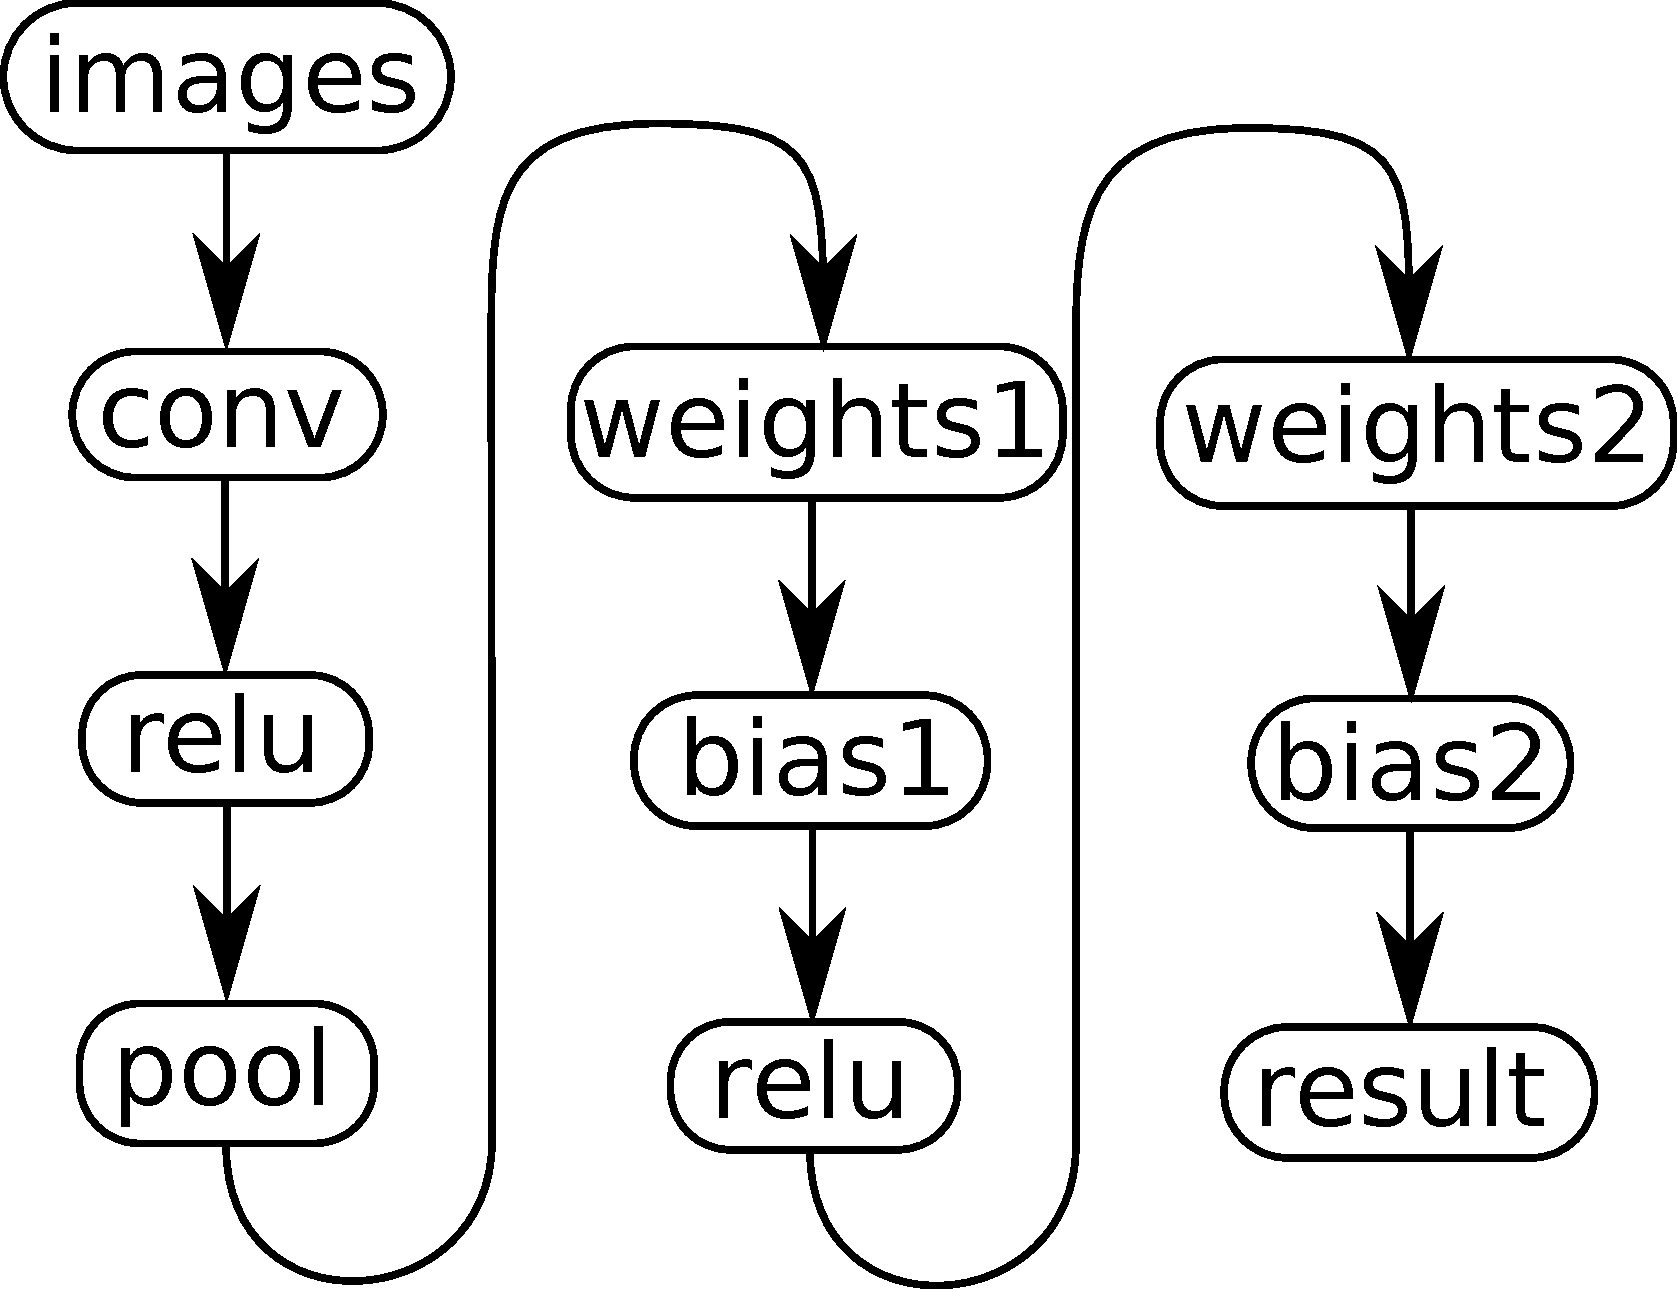
\includegraphics[width=0.6\textwidth]{figures/network}
	\caption{The network}
	\label{fig:network}
\end{figure}
\begin{enumerate}
	\begin{item}
		Figure~\ref{fig:network} describes the architecture of our CNN. We chose a small and therefore fast to train network, while still achieving high accuracy. We also tried larger networks through adding another conv-relu-pool layer and more hidden layers, with no improvement in accuracy but an increase in training time. The ReLu activation function was chosen because it performed better than tanh activation function.
	\end{item}
	\begin{item}
		The CNN was trained with standard parameters using softmax regression (\code{tf.nn.softmax\_cross\_entropy\_with\_logits}). This method applies a softmax nonlinearity to the output of the network and calculates the cross-entropy between the normalized predictions and a 1-hot encoding of the label. Various Optimizers were tested, with the Adam-Optimizer converging faster and to a higher accuracy compared to Momentum-Optimizer and Gradient-Descent-Optimizer.
	\end{item}

	\begin{item}
		The CNN had a very high success rate with an accuracy of 99\%, depending on the parameters. Figure~\ref{fig:wrong_preds} shows the predictions which were wrong. 
		\begin{figure}
			\centering	
			\begin{subfigure}[b]{0.45\textwidth}
				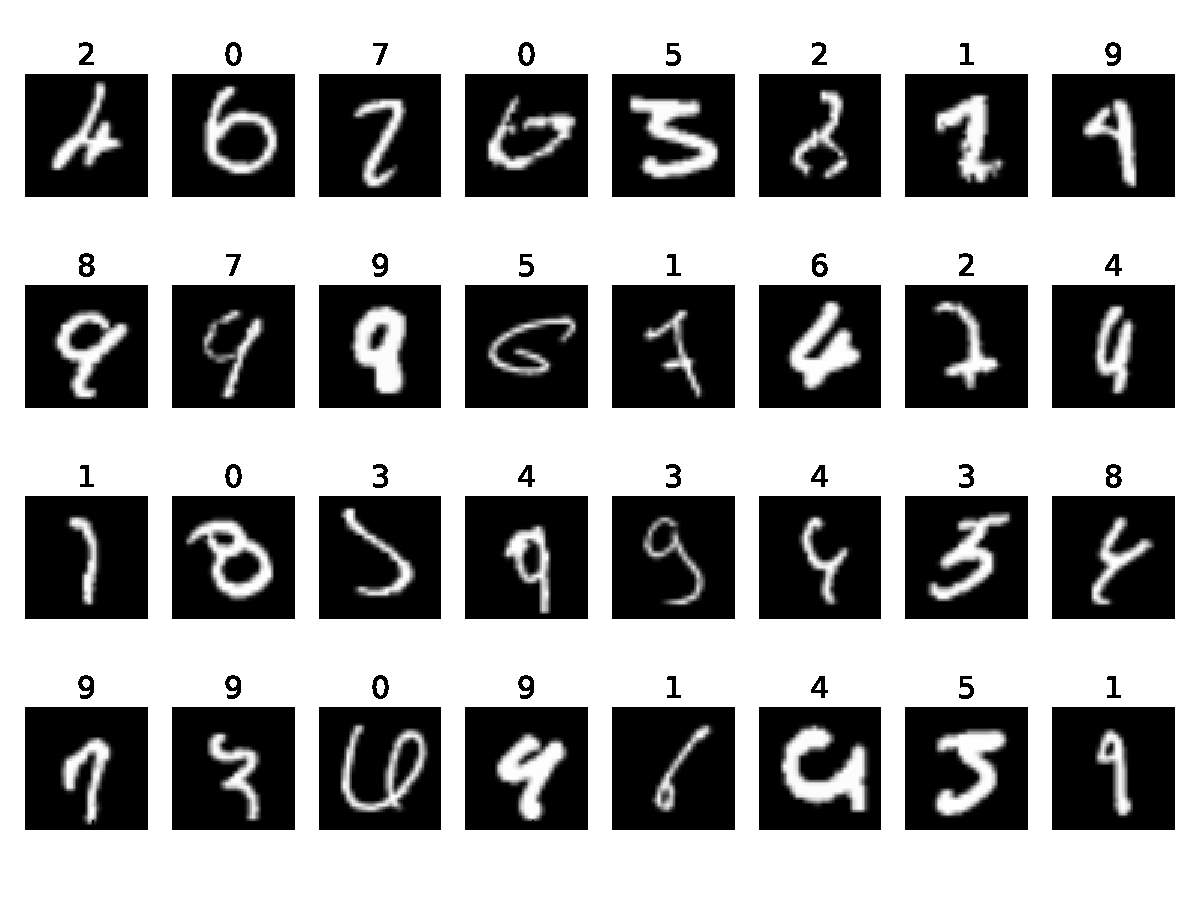
\includegraphics[width=\textwidth]{figures/wrong_predictions}
				\caption{wrong predictions}
				\label{fig:wrong_preds}
			\end{subfigure}	
			\begin{subfigure}[b]{0.45\textwidth}
				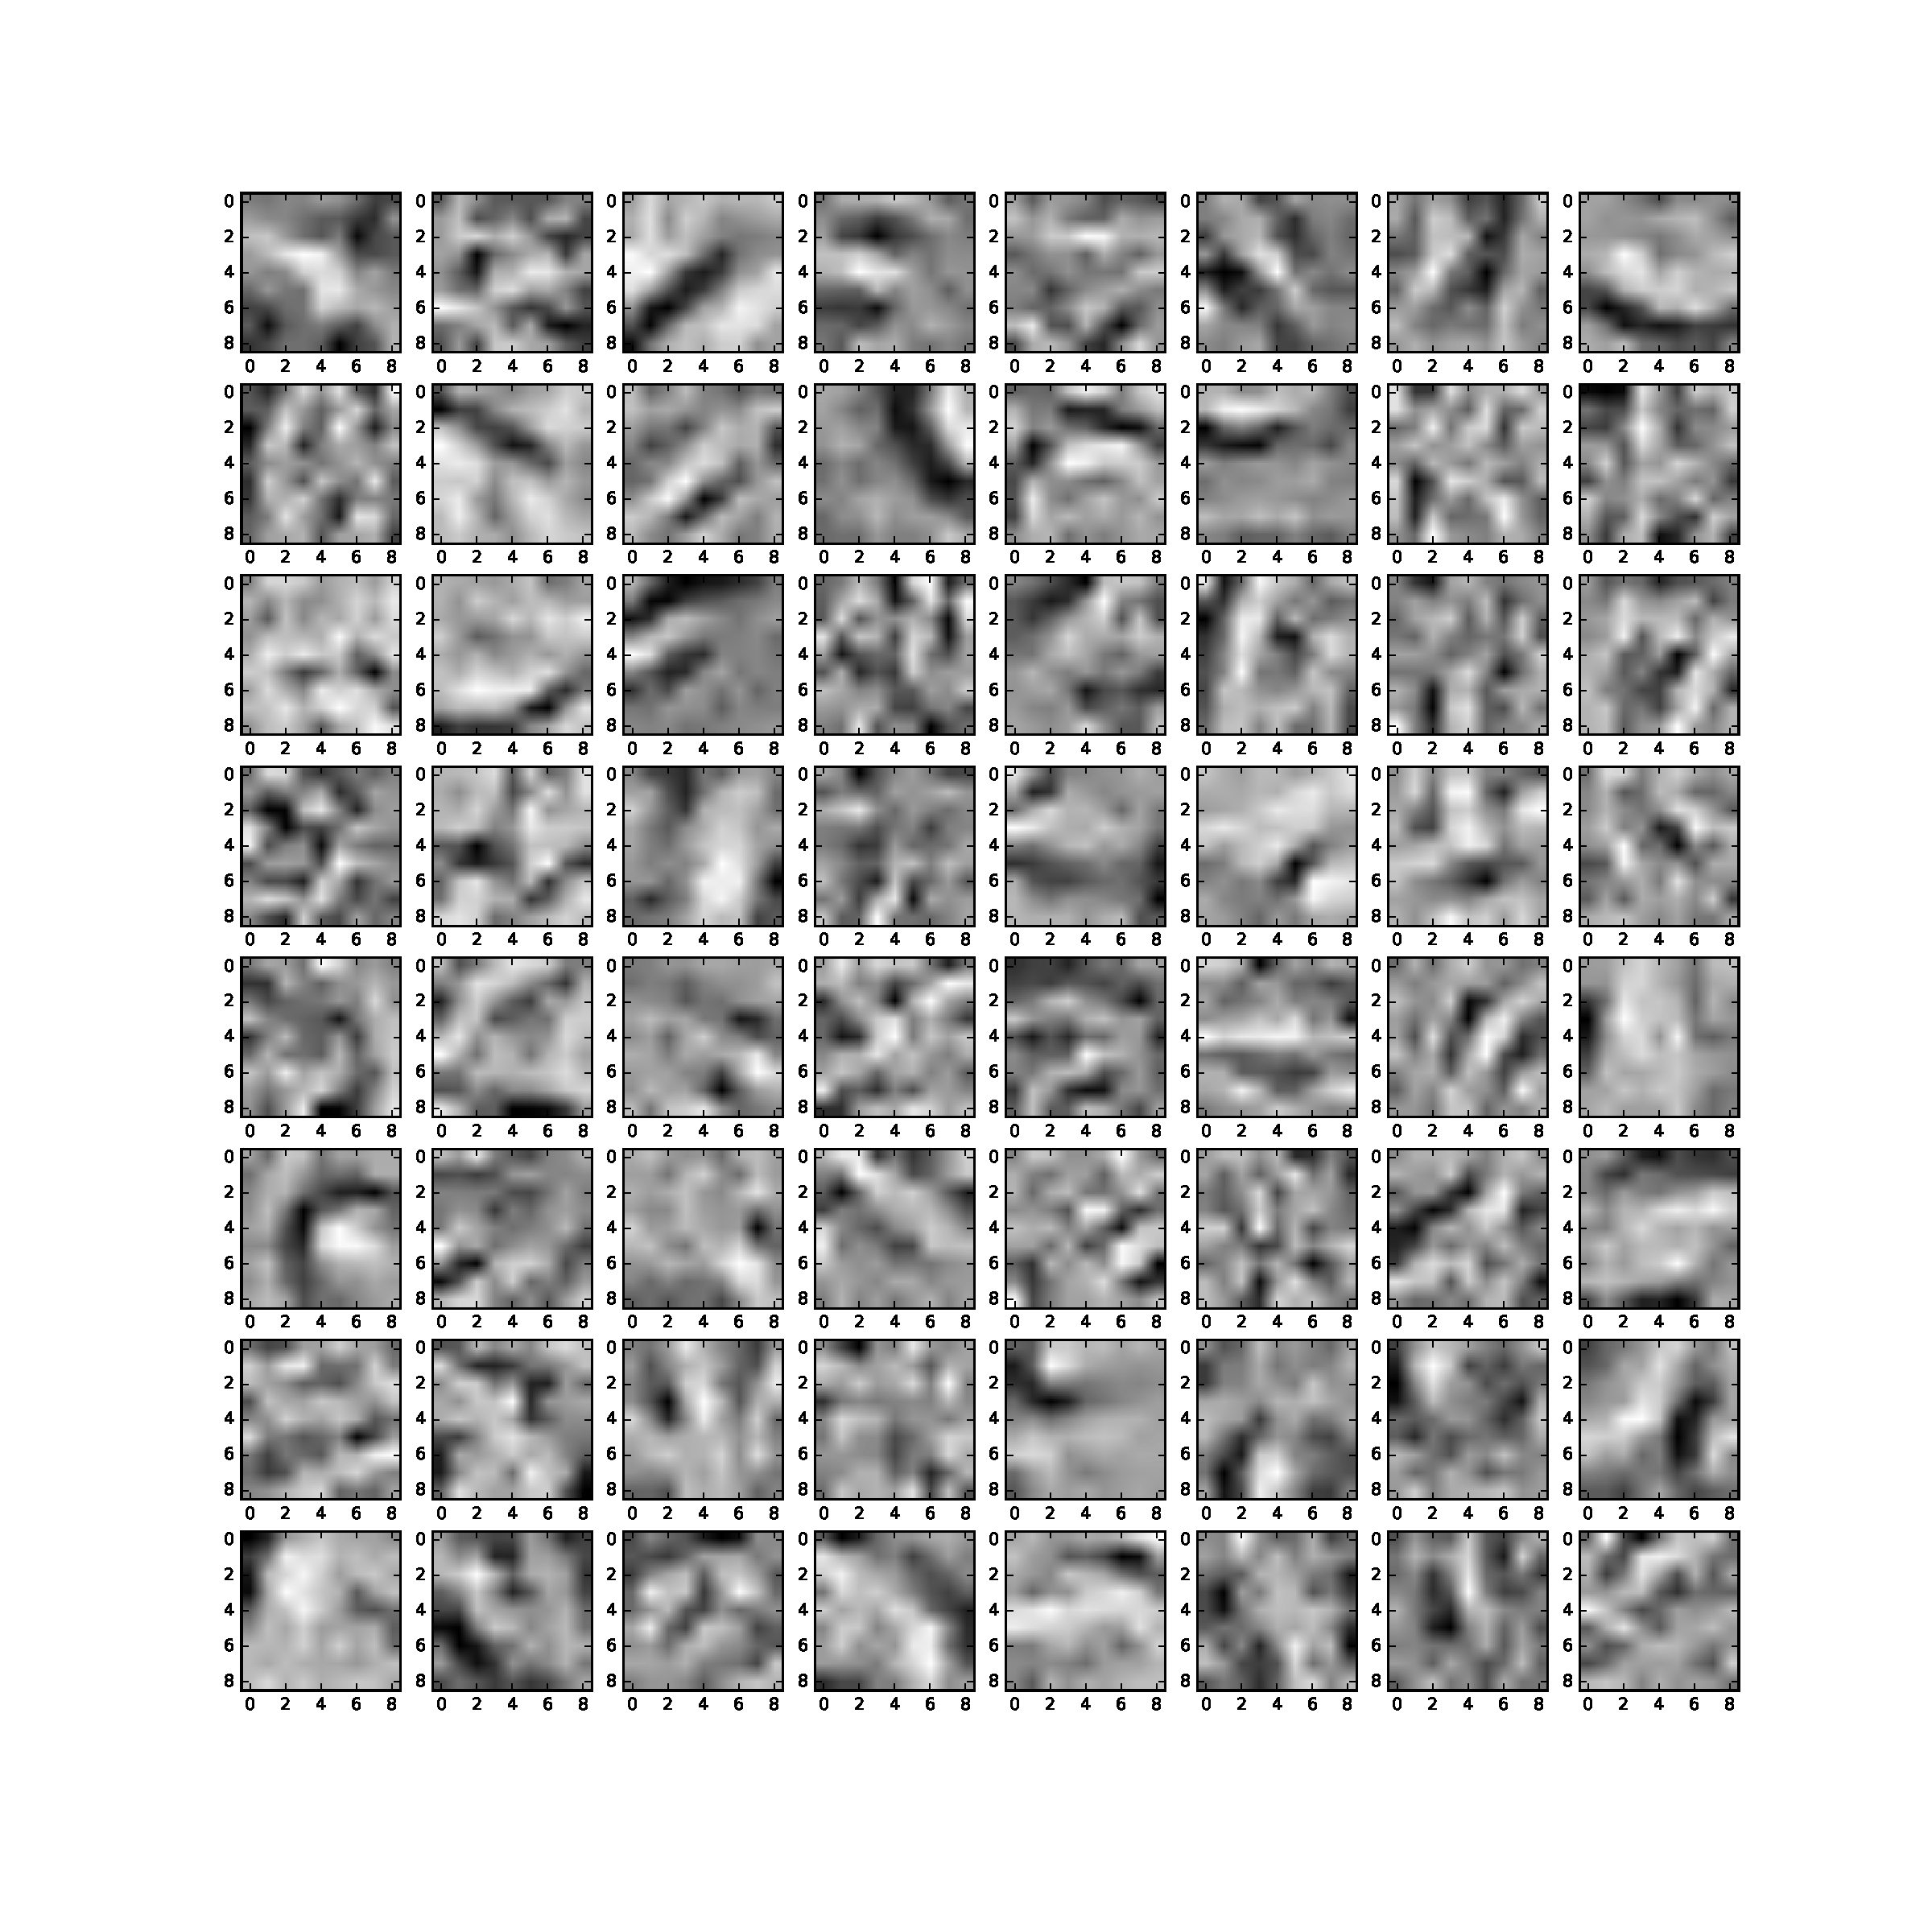
\includegraphics[width=\textwidth]{figures/99_43}
				\vspace{-24pt}
				\caption{visualization of CNN learning}
				\label{fig:vis_cnn}
			\end{subfigure}	
			\caption{visualizations for questions 3 and 7}
		\end{figure}
	\end{item}
\pagebreak
	\begin{item}
		No. While running solely on a CPU, setting the seed parameter for otherwise randomized initializations will give the same result for each run. The MNIST loader, which randomizes the batches per default, can be seeded via \code{np.random.seed}, while \code{tf.truncated\_normal} and \code{tf.nn.dropout} offer seed parameters. These efforts are of course futile while running on a GPU, since the high degree of multithreaded calculations will result in non-deterministic behaviour. 
	\end{item}
	\begin{item}
	For the evolution of accuracy with respect to the number of iterations, see 8. Training time on one million samples varied between 132 and 723 seconds on a GeForce GTX 1070, depending on the selection of the parameters.
	\end{item}

	\begin{item}
		Choosing a sensible learning rate is imperative. While a very small learning rate might take a long time to converge, a high learning rate might not reach the maximum accuracy at all. As seen in figure~\ref{fig:learning_rate}, choosing a rate of 0.001 is preferable to both 0.01 and 0.0001.
			\begin{figure}
				\centering	
				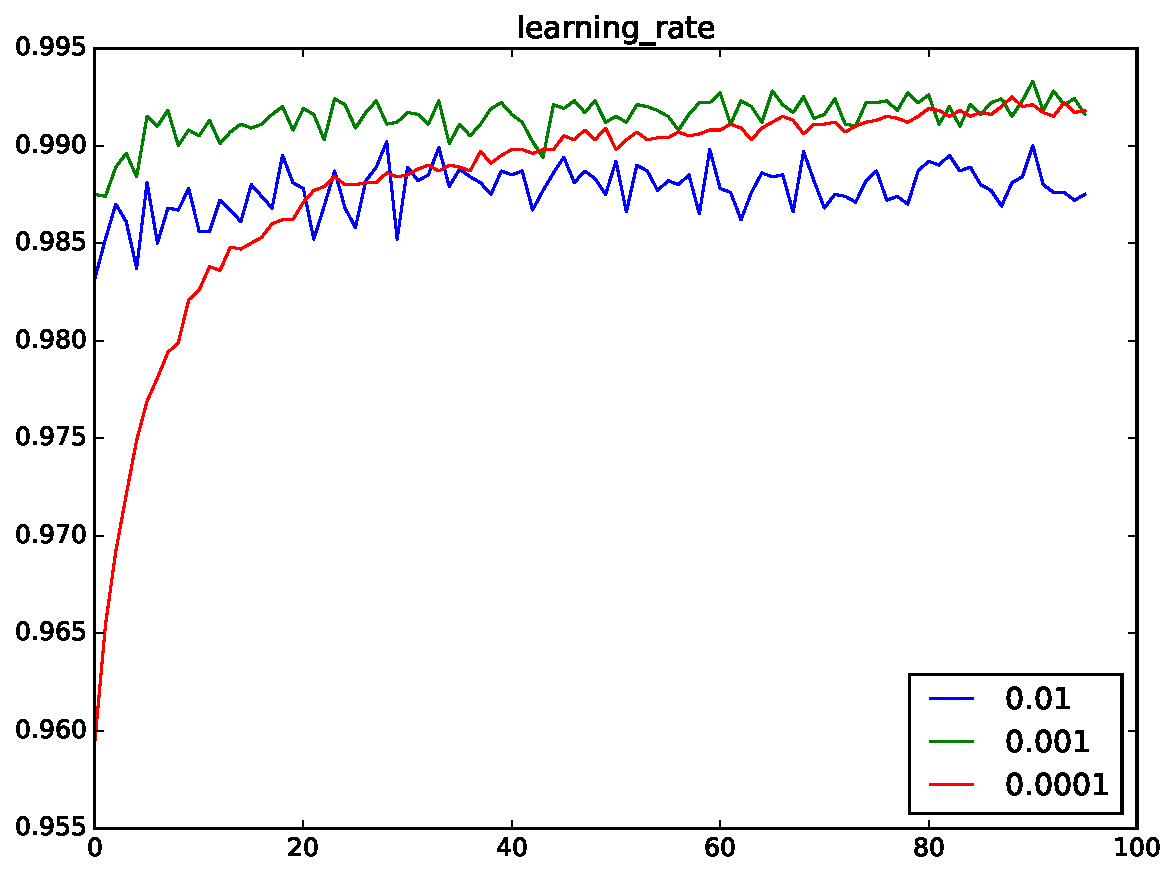
\includegraphics[width=0.7\textwidth]{figures/learning_rate}
				\caption{learning rate}
				\label{fig:learning_rate}
			\end{figure}

	\end{item}
	\begin{item}
		A CNN basically trains a feature extractor which is then used to classify any given data, preferably of the same type as the training data, in our case images. Figure~\ref{fig:vis_cnn} shows a visualization of these features.
	\end{item}
	\begin{item}
		\begin{figure}
			\centering
			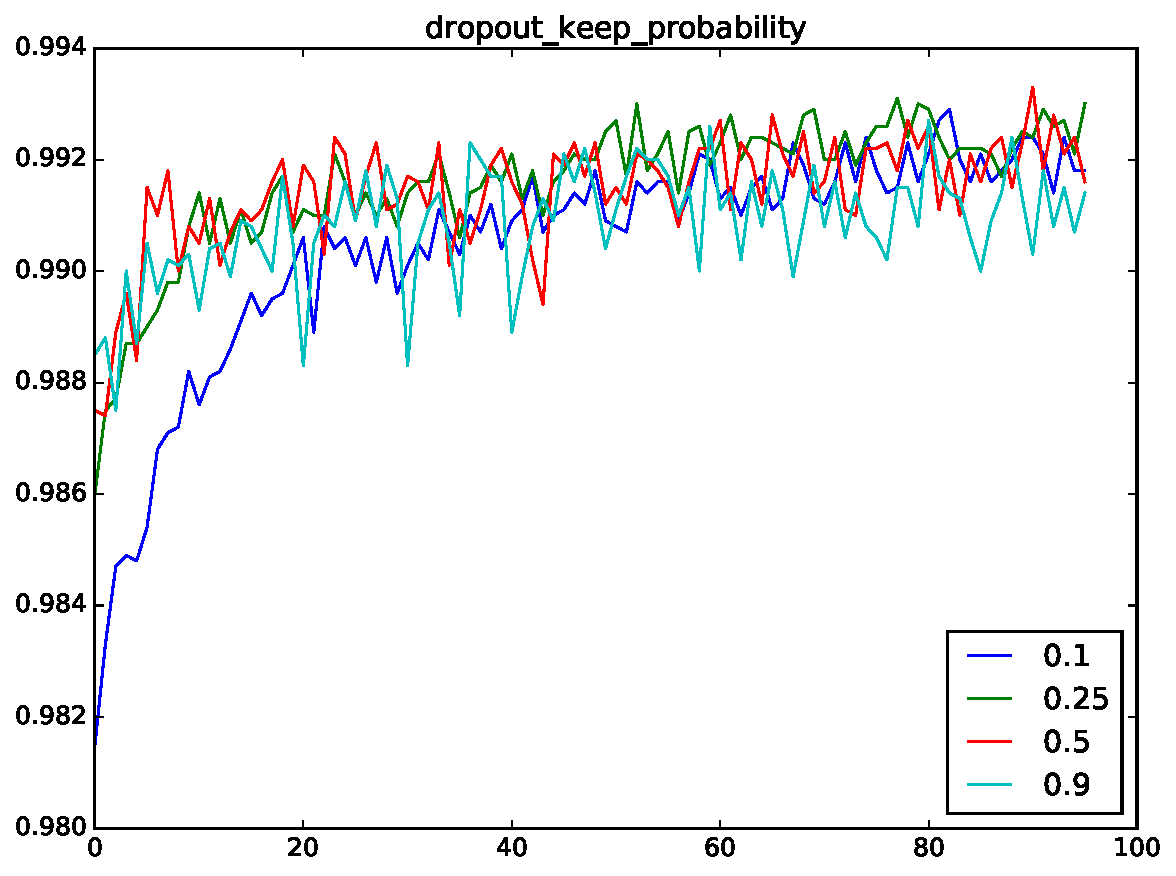
\includegraphics[width=0.3\textwidth]{figures/dropout_keep_probability}
			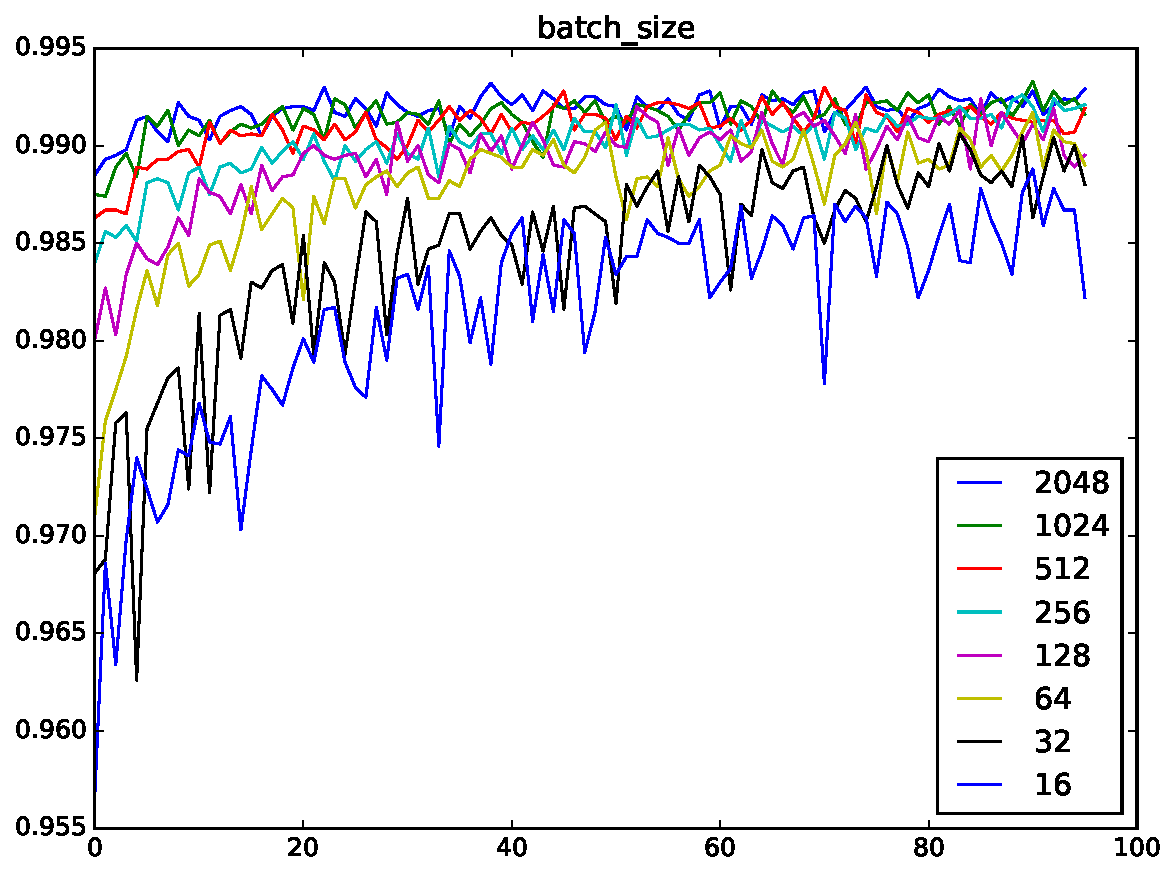
\includegraphics[width=0.3\textwidth]{figures/batch_size}
			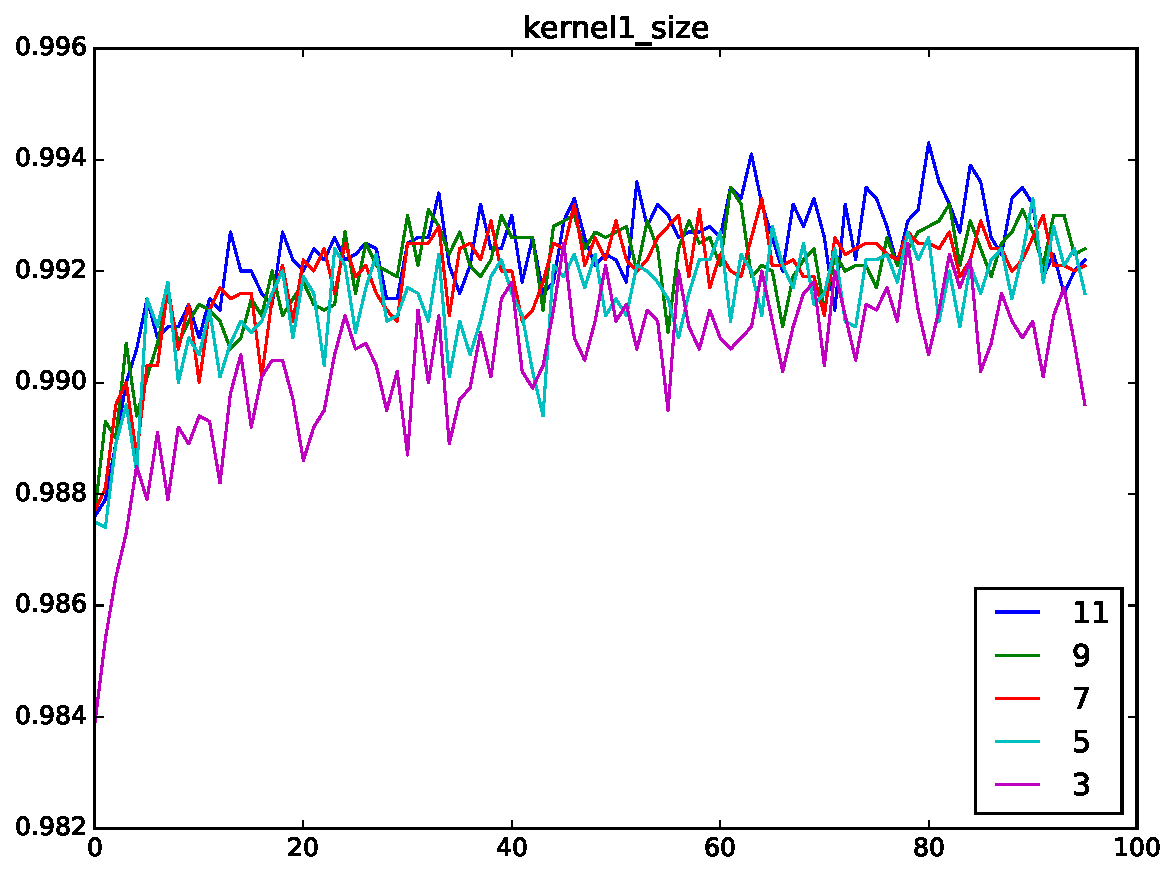
\includegraphics[width=0.3\textwidth]{figures/kernel1_size}
			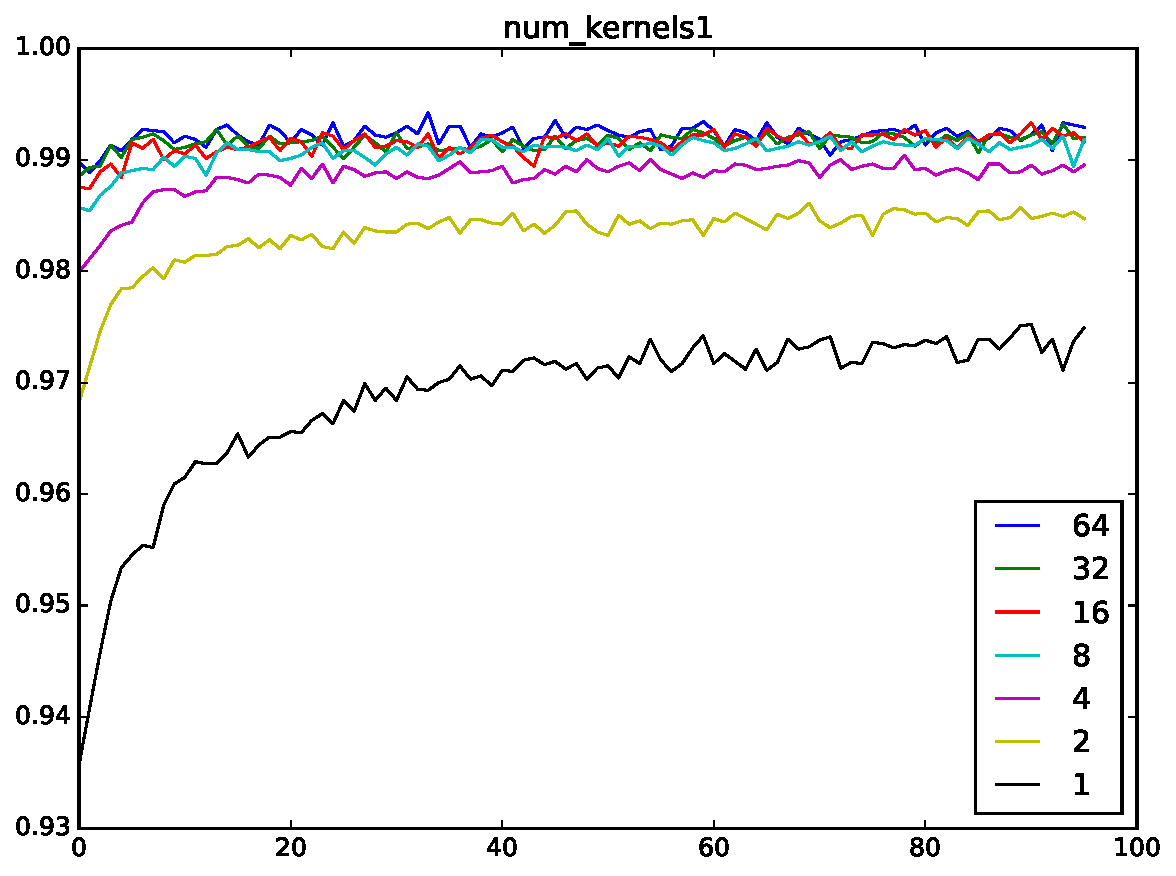
\includegraphics[width=0.3\textwidth]{figures/num_kernels1}
			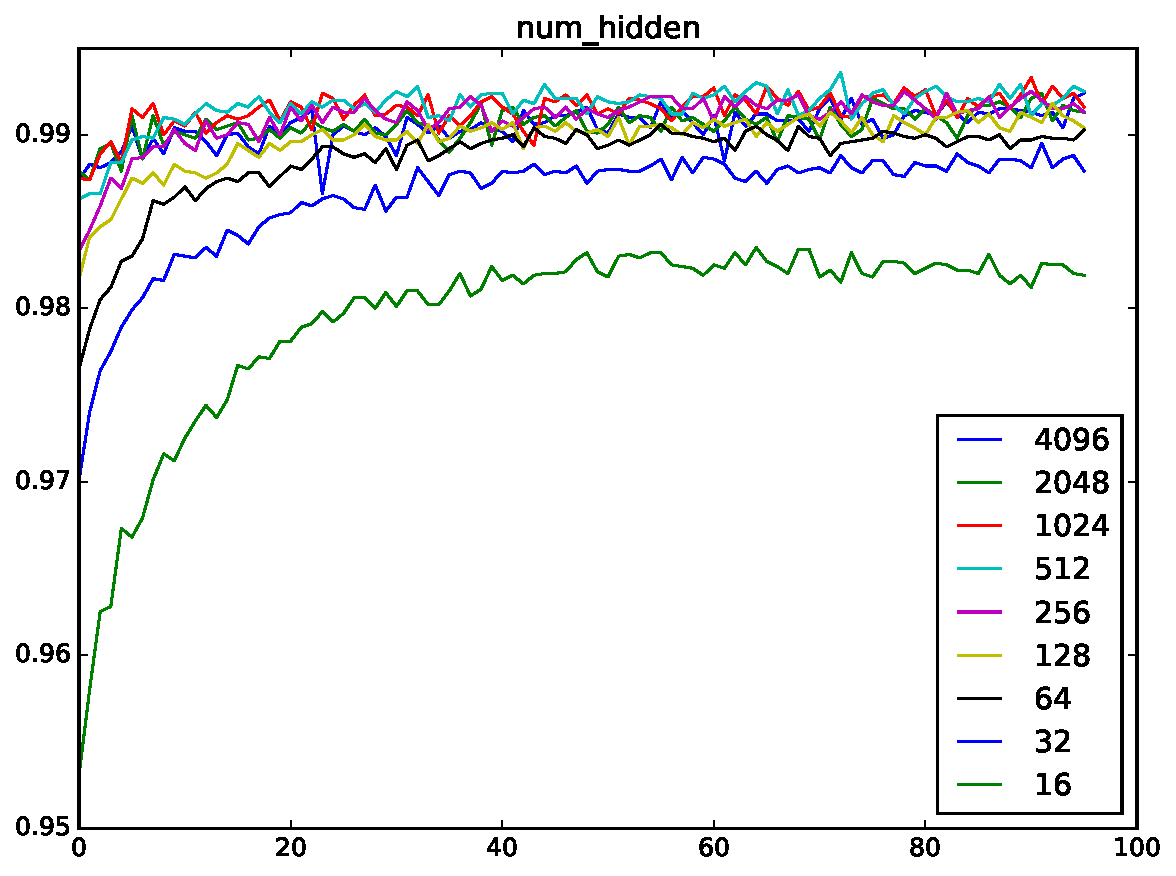
\includegraphics[width=0.3\textwidth]{figures/num_hidden}
			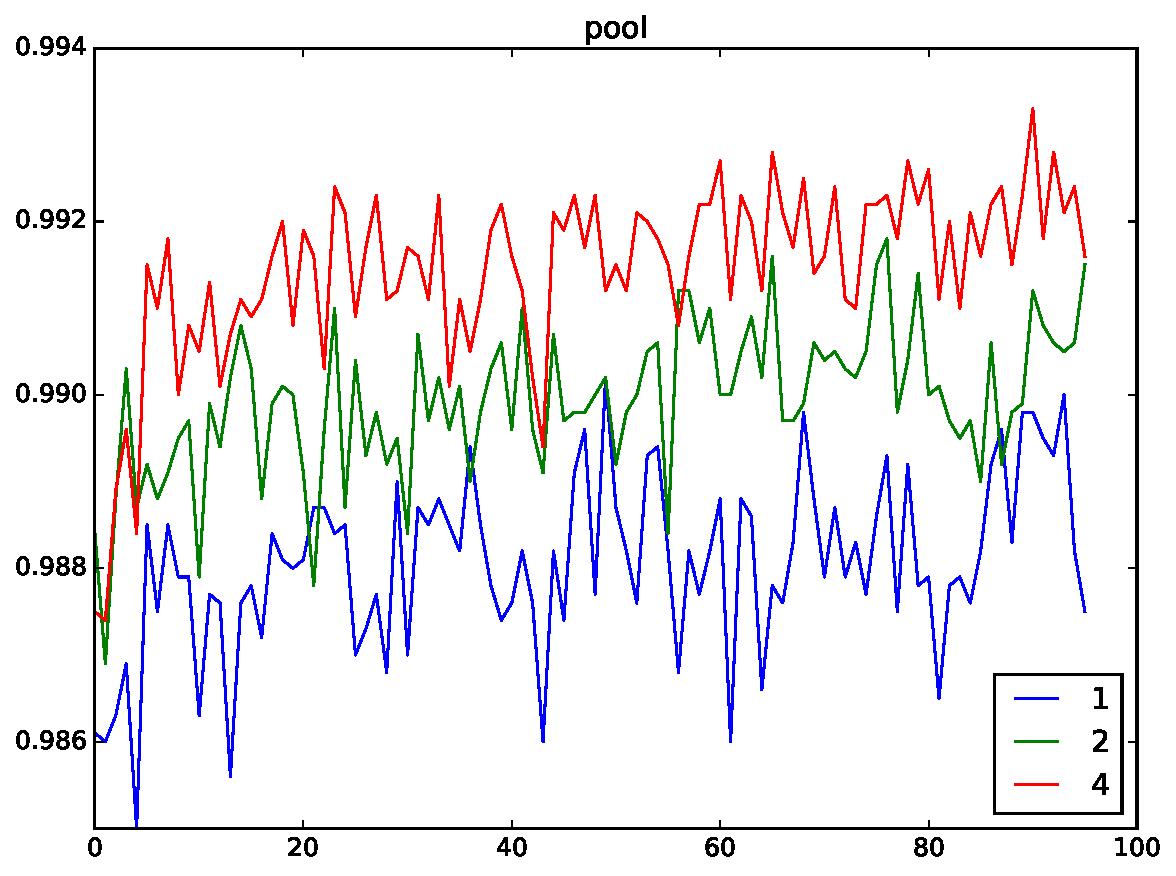
\includegraphics[width=0.3\textwidth]{figures/pool}
			\caption{parameter comparison}
			\label{fig:parameters}
		\end{figure}
		Figure~\ref{fig:parameters} details the accuracy in respect to various parameter changes. For the batch size and the number of kernels, a higher value results in better accuracy. While this is also the case for the kernel size, the calculation is more costly. The calculation time needed for a kernel size of 5 doubles the kernel size of 3. For the pooling, the best results are achieved with a value of 4. This seems to be the maximum, though, since additional tests have shown that an even higher value of 7 or even 14 have a much lower rated result.
		The dropout keep probability shows the best results for a value of 0.25. 
		
	\end{item}
	\begin{item}
		Table \ref{smallest_conf} shows two acceptable but small configurations.
		\begin{table}[h]
			\caption{Minimal configurations}
			\label{smallest_conf}
			\centering
			\begin{tabular}{lll}
				\toprule
				Parameter     & Accuracy 97.4\%     & Accuracy 99\% \\
				\midrule
				num\_hidden & 64 & 512 \\
				num\_kernels1 & 4 & 16 \\
				learning\_rate & 0.001 & 0.001 \\
				regularization\_factor & 0.0001 & 0.0001 \\
				batch\_size & 2048 & 512 \\
				dropout\_keep\_probability & 0.25 & 0.25 \\
				seed & 666 & 666 \\
				kernel1\_size & 3 & 5 \\
				test\_interval & 100 & 100 \\
				num\_batches & 20001 & 2001 \\
				pool & 4 & 4 \\
				
				
				\bottomrule
			\end{tabular}
		\end{table}
	\end{item}
	\begin{item}
		Table \ref{pooling_comp_table} depicts the different pooling kernel sizes and its consequences. A kernel size of 1 is the equivalent to no pooling.
		
		\begin{figure}[h]
			\centering	
			\begin{subfigure}[b]{0.45\textwidth}
				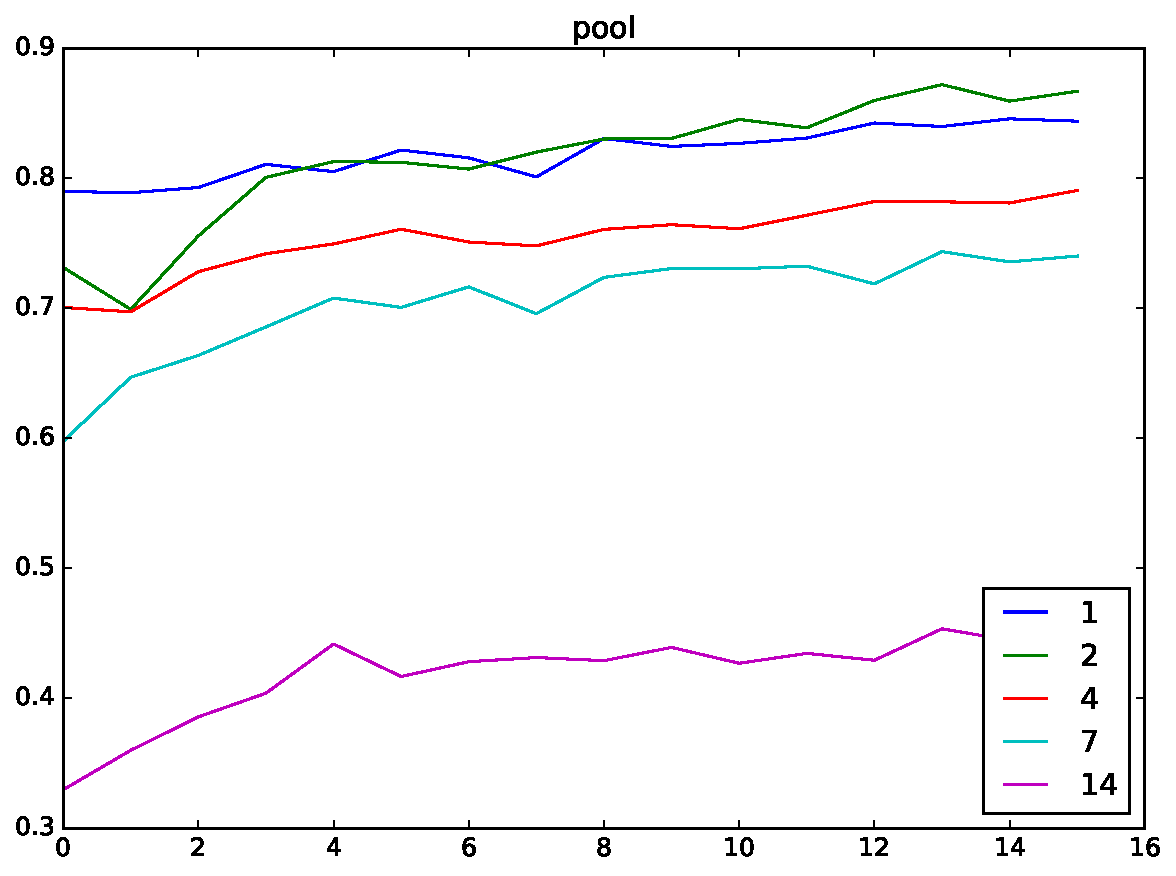
\includegraphics[width=\textwidth]{figures/pool_cpu}
				\caption{the plot}
				\label{fig:pooling_cpu}
			\end{subfigure}	
			\quad
			\begin{subtable}[b]{0.4\textwidth}
				\begin{tabular}{lll}
					\toprule
					Pooling Kernel Size     & Seconds & Accuracy \\
					\midrule
					1 & 261.9 & 0.8438 \\
					2 & 255.7 & 0.8668 \\
					4 & 214.0 & 0.7905 \\
					7 & 211.8 & 0.7401 \\
					14 & 209.5 & 0.454 \\
					\bottomrule
					%		\vspace{1pt}
				\end{tabular}
				\caption{the table}
				\label{pooling_comp_table}
			\end{subtable}	
			\caption{pooling comparisons}
			\label{pooling_comparisons}
		\end{figure}
	\end{item}

	
\end{enumerate}

\end{document}
